\documentclass[12pt,a4paper]{article}
\usepackage[margin=2.5cm]{geometry}
\usepackage{amsmath, amssymb}
\usepackage{graphicx}
\usepackage{booktabs}
\usepackage{float}
\usepackage{parskip}
\usepackage[most]{tcolorbox}
\usepackage{fancyhdr}
\usepackage{setspace}
\usepackage{cite}
\usepackage{hyperref}

% ---------------------------------------------------------------
% NOTE FOR OVERLEAF:
%   Upload  Fig-1.png  (or Fig-1.pdf) to the same folder as this
%   .tex file. LaTeX will find it automatically via \graphicspath.
%   PDF is preferred (vector, scales perfectly); PNG also works.
% ---------------------------------------------------------------
\graphicspath{{./}}          % look in the same directory as the .tex

\pagestyle{fancy}
\fancyhf{}
\lhead{Condensed Matter Physics -- Assignment}
\rhead{2D Point Groups}
\cfoot{\thepage}
\setlength{\headheight}{14pt}

\setlength{\parskip}{6pt}

\begin{document}

\begin{center}
  {\Large \textbf{Assignment: 2D Crystallographic Point Groups}} \\[6pt]
  {\large Condensed Matter Physics}
\end{center}

\vspace{4pt}
\hrule
\vspace{10pt}

% --------------------------------------------------------
\section*{The basic idea}

The problem is to find all the point groups compatible with a 2D periodic lattice.
The key constraint comes from the fact that any rotation $R(\theta)$ must map lattice
vectors to lattice vectors. In the lattice basis, $R$ has integer entries, so its trace
must be an integer \cite{Kittel2005, Ashcroft1976}:
\[
  \mathrm{tr}\, R = 2\cos\theta \in \mathbb{Z}
\]
This only works for $\cos\theta \in \{0, \pm\tfrac{1}{2}, \pm 1\}$, which gives
$\theta = 0^\circ, 60^\circ, 90^\circ, 120^\circ, 180^\circ$, or equivalently
$n = 1, 2, 3, 4, 6$. So pentagons are out -- you simply can't tile a plane
with 5-fold symmetry and keep a lattice \cite{Kittel2005}.

The full list in Schoenflies notation is \cite{Bradley1972, Burns1990}:
\[
  C_1,\; C_2,\; C_3,\; C_4,\; C_6 \quad \text{(rotation only)}
\]
\[
  D_1,\; D_2,\; D_3,\; D_4,\; D_6 \quad \text{(rotation + mirrors)}
\]
That's 10 point groups total.

% --------------------------------------------------------
\section*{How I'm constructing them: the motif trick}

In class we did the dice thing -- you place a motif at every Bravais lattice point,
and the symmetry of the whole pattern is determined by \emph{both} the lattice
\emph{and} how you shade (mark) the motif \cite{Hammond2015}. The idea is:

\begin{itemize}
  \item Put dots \textbf{off} all mirror lines $\to$ no mirrors survive $\to$ you get a
        cyclic group $C_n$.
  \item Put dots \textbf{on} the mirror lines symmetrically $\to$ mirrors preserved
        $\to$ you get a dihedral group $D_n$.
\end{itemize}

Each Bravais lattice has a maximum point group symmetry, and by shading
you can realise any subgroup of that \cite{Ashcroft1976, Hammond2015}:

\begin{center}
\begin{tabular}{lcc}
\toprule
Lattice & Max symmetry & Motif \\
\midrule
Oblique & $C_2$ & parallelogram \\
Rectangular & $D_2$ & rectangle \\
Centred rectangular & $D_2$ & rectangle \\
Square & $D_4$ & square \\
Hexagonal & $D_6$ & hexagon / triangle \\
\bottomrule
\end{tabular}
\end{center}

Below is a summary figure (Fig.~\ref{fig:pointgroups}) of all 10 groups,
then I go through each one.

% ---------------------------------------------------------------
% FIGURE 1  -- external file: Fig-1.png (or Fig-1.pdf)
% Upload Fig-1.png / Fig-1.pdf to Overleaf alongside this .tex file.
% ---------------------------------------------------------------
\begin{figure}[H]
  \centering
  \fbox{%
    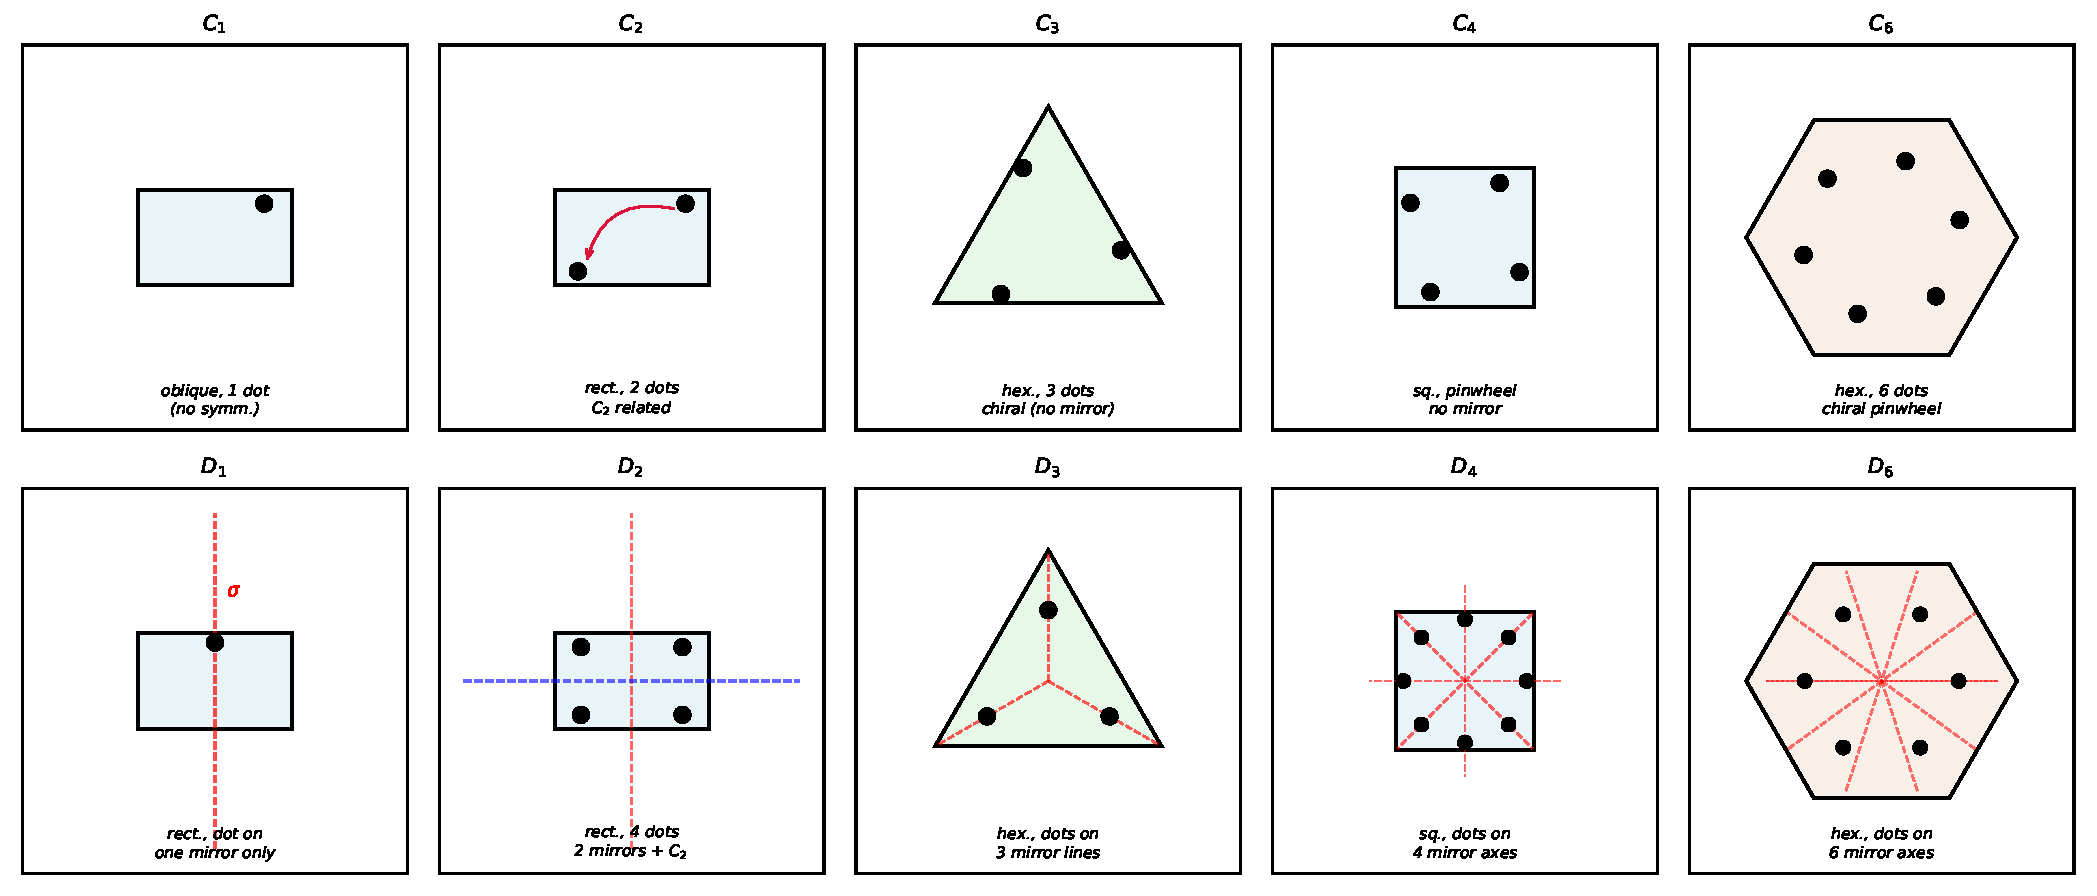
\includegraphics[width=0.97\linewidth]{Fig-1}%
  }
  \caption{%
    All 10 two-dimensional crystallographic point groups illustrated using
    the lattice$+$motif (shaded-basis) method \cite{Hammond2015, Kittel2005}.
    Each panel shows a motif (rectangle / square / triangle / hexagon) placed
    at a Bravais lattice point; filled circles indicate the shading of the motif.
    \textit{Top row} ($C_1$--$C_6$): cyclic groups -- dots placed \emph{off}
    all mirror lines, so only $n$-fold rotation survives.
    \textit{Bottom row} ($D_1$--$D_6$): dihedral groups -- dots placed
    \emph{on} the mirror axes (red dashed lines), preserving both rotations
    and reflections.
    Figure generated with Python/Matplotlib \cite{Hunter2007};
    script: \texttt{generate\_fig1.py} (provided separately).%
  }
  \label{fig:pointgroups}
\end{figure}

% --------------------------------------------------------
\newpage
\section*{Going through each group}

\subsection*{$C_1$ -- no symmetry (identity only)}

Take an oblique lattice and put a single dot at a completely random position inside the
motif -- not on any axis, not on any mirror. The only thing that maps this pattern to
itself is the identity ($360^\circ$ rotation). No $C_2$, no mirrors. This is the
``trivial'' point group, everything has at least $C_1$ symmetry \cite{Burns1990}.

\[
\boxed{\text{Oblique lattice} + \text{single asymmetric dot} \;\Rightarrow\; C_1}
\]

\subsection*{$C_2$ -- 2-fold rotation, no mirrors}

Use a rectangular lattice. Place two dots inside the rectangle, related to each other
by a $180^\circ$ rotation about the centre. The crucial thing is to put them
\emph{off} the horizontal and vertical mirror lines -- if either dot sat on a mirror,
you'd have $D_1$ or $D_2$ instead. With this asymmetric placement the $C_2$ rotation
maps dot~1 to dot~2 and back, but no reflection does \cite{Kittel2005}. Group order = 2.

\[
\boxed{\text{Rectangular lattice} + \text{two dots related by }C_2\text{, off all mirrors} \;\Rightarrow\; C_2}
\]

\subsection*{$C_3$ -- 3-fold rotation, no mirrors}

Switch to a hexagonal (triangular) lattice. Use a triangular motif and place three
dots arranged in a small \emph{chiral} triangle inside it -- i.e.\ the inner triangle
is rotated relative to the outer one, so none of the three dots sits on any altitude
(which would be a mirror line). Each dot maps to the next by $120^\circ$. No mirror
survives \cite{Hammond2015}.

\[
\boxed{\text{Hex. lattice} + \text{chiral 3-dot motif} \;\Rightarrow\; C_3}
\]

\subsection*{$C_4$ -- 4-fold rotation, no mirrors}

Square lattice, square motif. Arrange four dots in a pinwheel pattern -- like a
swastika shape -- each related to the next by $90^\circ$. The key: rotate the whole
pattern by $45^\circ$ so that none of the dots lands on the four mirror lines of the
square ($x$-axis, $y$-axis, and the two diagonals). The $C_4$ axis is there, all
four mirrors are broken \cite{Ashcroft1976}. Group order = 4.

\[
\boxed{\text{Square lattice} + \text{pinwheel 4-dot motif} \;\Rightarrow\; C_4}
\]

\subsection*{$C_6$ -- 6-fold rotation, no mirrors}

Hexagonal lattice, hexagonal motif. Six dots in a pinwheel: each is related to the
next by $60^\circ$, but the whole arrangement is rotated slightly so none of the dots
sits on any of the six mirror lines of the hexagon \cite{Hammond2015}. Group order = 6.

\[
\boxed{\text{Hex. lattice} + \text{pinwheel 6-dot motif} \;\Rightarrow\; C_6}
\]

\subsection*{$D_1$ -- one mirror, no rotation (other than identity)}

Rectangular lattice again. Now place a single dot exactly on the \emph{vertical}
mirror line of the rectangle, but \emph{not} on the horizontal one. The vertical
mirror maps the dot to itself (fine). The horizontal mirror would move the dot to
a different height -- broken. The $C_2$ would put a second dot at the mirror
image through the centre -- also broken. So we're left with just one mirror. This
is the same as $C_{1v}$ in some notations \cite{Bradley1972}. Group order = 2.

\[
\boxed{\text{Rect. lattice} + \text{dot on one mirror only} \;\Rightarrow\; D_1}
\]

\subsection*{$D_2$ -- 2-fold rotation + 2 mirror lines}

Rectangular lattice. Place four dots, one in each quadrant, symmetrically:
$(x_0, y_0)$, $(-x_0, y_0)$, $(x_0, -y_0)$, $(-x_0, -y_0)$. Now both mirrors
(horizontal and vertical) are preserved, and the $C_2$ rotation is also a symmetry
(it maps each dot to the one diagonally opposite). The full symmetry of the
rectangle is restored \cite{Kittel2005}. Group order = 4.

\[
\boxed{\text{Rect. lattice} + \text{4 dots symmetric in both mirrors} \;\Rightarrow\; D_2}
\]

\subsection*{$D_3$ -- 3-fold rotation + 3 mirror lines}

Hexagonal lattice, triangular motif. Place one dot on each of the three altitude lines
of the equilateral triangle (the mirror lines). The $C_3$ rotation cycles the three
dots, and each of the three mirrors maps the dot on its line to itself and swaps the
other two. Everything is preserved. This group is isomorphic to $S_3$, the symmetric
group on 3 elements \cite{Burns1990, Bradley1972}. Group order = 6.

\[
\boxed{\text{Hex. lattice} + \text{3 dots on the 3 altitudes} \;\Rightarrow\; D_3}
\]

\subsection*{$D_4$ -- 4-fold rotation + 4 mirror lines}

Square lattice. The square has 4 mirror lines: the $x$-axis, $y$-axis, and the two
diagonals. Place dots symmetrically on all four of them (one dot per mirror axis,
all at the same radius from centre). The $C_4$ rotation cycles the dots on adjacent
mirrors, so it's a symmetry. All 4 mirrors are preserved \cite{Ashcroft1976}. Group order = 8.

\[
\boxed{\text{Square lattice} + \text{dots on all 4 mirror axes} \;\Rightarrow\; D_4}
\]

\subsection*{$D_6$ -- 6-fold rotation + 6 mirror lines}

Hexagonal lattice, hexagonal motif. The hexagon has 6 mirror lines (3 through
opposite vertices, 3 through midpoints of opposite edges). Place one dot on each
mirror line at equal radius. The $C_6$ rotation cycles all 6 dots, and all 6 mirrors
are preserved. This is the largest 2D crystallographic point group \cite{Hammond2015}. Group order = 12.

\[
\boxed{\text{Hex. lattice} + \text{dots on all 6 mirror axes} \;\Rightarrow\; D_6}
\]

% --------------------------------------------------------
\newpage
\section*{Summary}

\begin{center}
\renewcommand{\arraystretch}{1.35}
\begin{tabular}{ccccp{4.5cm}}
\toprule
\textbf{Group} & \textbf{$n$-fold rotation} & \textbf{No.\ of mirrors} & \textbf{Order} & \textbf{Lattice} \\
\midrule
$C_1$  & 1 & 0 & 1  & Oblique \\
$C_2$  & 2 & 0 & 2  & Oblique / rectangular \\
$C_3$  & 3 & 0 & 3  & Hexagonal \\
$C_4$  & 4 & 0 & 4  & Square \\
$C_6$  & 6 & 0 & 6  & Hexagonal \\
\midrule
$D_1$  & 1 & 1 & 2  & Rectangular \\
$D_2$  & 2 & 2 & 4  & Rectangular \\
$D_3$  & 3 & 3 & 6  & Hexagonal \\
$D_4$  & 4 & 4 & 8  & Square \\
$D_6$  & 6 & 6 & 12 & Hexagonal \\
\bottomrule
\end{tabular}
\end{center}

\vspace{6pt}
A few things worth noting:
\begin{itemize}
  \item $C_n \subset D_n$ always -- the dihedral group contains the cyclic group as a
        subgroup (the rotations).
  \item The order of $D_n$ is $2n$ because you have $n$ rotations and $n$ mirror reflections.
  \item $C_5, C_7, C_8, \ldots$ are perfectly fine abstract groups, but they are \emph{not}
        crystallographic -- no periodic lattice can support them, because $2\cos(2\pi/5)$
        and similar values are irrational, not integers \cite{Kittel2005, Ashcroft1976}.
  \item Quasicrystals (e.g.\ the Al-Mn alloy discovered by Shechtman in 1982 \cite{Shechtman1984}) \emph{do}
        show 5-fold diffraction patterns, but they are not periodic lattices -- they are
        quasiperiodic.
\end{itemize}

% --------------------------------------------------------
\begin{thebibliography}{9}

\bibitem{Kittel2005}
C.~Kittel,
\textit{Introduction to Solid State Physics}, 8th ed.
Wiley, Hoboken, NJ, 2005.
(Ch.~1: Crystal Structure; crystallographic restriction and Bravais lattices.)

\bibitem{Ashcroft1976}
N.~W.~Ashcroft and N.~D.~Mermin,
\textit{Solid State Physics}.
Holt, Rinehart and Winston, New York, 1976.
(Ch.~7: Classification of Bravais lattices and crystal structures.)

\bibitem{Bradley1972}
C.~J.~Bradley and A.~P.~Cracknell,
\textit{The Mathematical Theory of Symmetry in Solids}.
Clarendon Press, Oxford, 1972.
(Complete tables of point groups in Schoenflies and international notation.)

\bibitem{Burns1990}
G.~Burns and A.~M.~Glazer,
\textit{Space Groups for Solid State Scientists}, 2nd ed.
Academic Press, San Diego, 1990.
(Ch.~2: Point groups and their relation to lattice symmetry.)

\bibitem{Hammond2015}
C.~Hammond,
\textit{The Basics of Crystallography and Diffraction}, 4th ed.
Oxford University Press, Oxford, 2015.
(Ch.~2--4: The lattice$+$motif construction for point and space groups.)

\bibitem{Shechtman1984}
D.~Shechtman, I.~Blech, D.~Gratias, and J.~W.~Cahn,
``Metallic phase with long-range orientational order and no translational symmetry,''
\textit{Phys.\ Rev.\ Lett.}, \textbf{53}, 1951 (1984).
(Discovery of icosahedral 5-fold symmetry in Al--Mn quasicrystals.)

\bibitem{Hunter2007}
J.~D.~Hunter,
``Matplotlib: A 2D graphics environment,''
\textit{Computing in Science \& Engineering}, \textbf{9}(3), 90--95 (2007).
(Fig.~\ref{fig:pointgroups} generated using Matplotlib; script \texttt{generate\_fig1.py}.)

\end{thebibliography}

\end{document}
